\section{Introduction}

\begin{frame}{Why Performance Profiling Matters}
    \begin{columns}
        \begin{column}{0.6\textwidth}
            \begin{itemize}
                \item \textbf{Performance Bottlenecks} are often not where you think
                \item \textbf{Optimization without data} leads to wasted effort
                \item \textbf{Scalability Issues} appear with larger data sets or systems
            \end{itemize}
            
        \end{column}
        \begin{column}{0.4\textwidth}
            \centering
            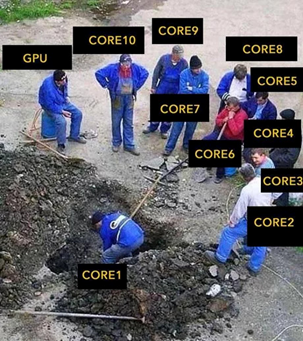
\includegraphics[width=\textwidth]{img/intro1.png}
        \end{column}
    \end{columns}
\end{frame}

\begin{frame}{Real World Example}
  \textbf{m5C-RNA}:
  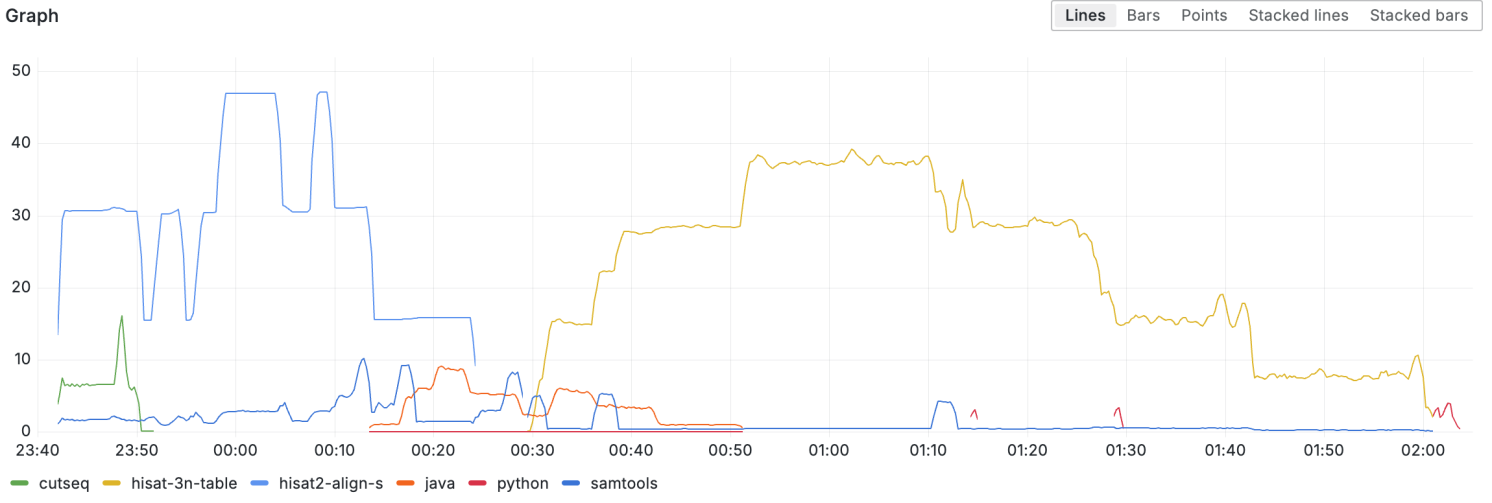
\includegraphics[width=\textwidth]{img/rna.png}
\end{frame}

\begin{frame}{Real World Example}
    \begin{itemize}
        \item Profiling of a HPC application
    \end{itemize}
    
    \begin{columns}
        \begin{column}{0.5\textwidth}
            \centering
            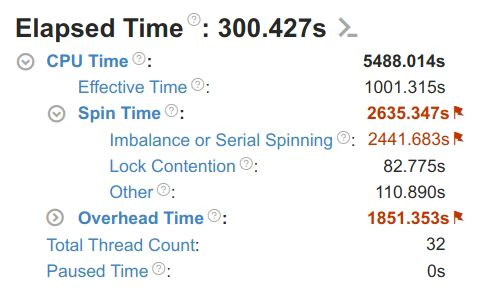
\includegraphics[width=\textwidth]{img/example1.jpg}
        \end{column}
        \begin{column}{0.5\textwidth}
            \centering
            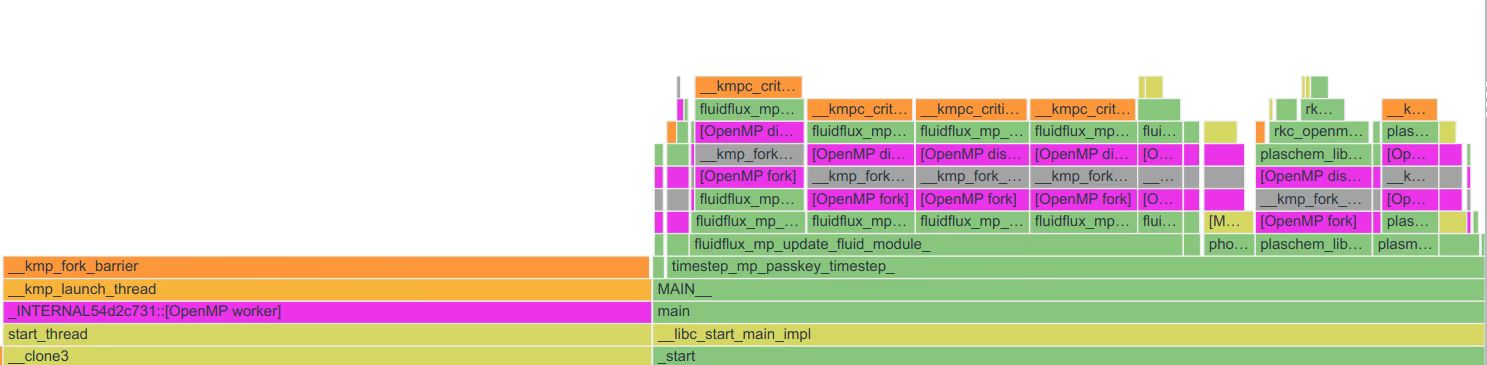
\includegraphics[width=\textwidth]{img/example2.jpg}
        \end{column}
    \end{columns}
\end{frame}

\begin{frame}{Profiling vs. Guessing}
    \begin{columns}
        \begin{column}{0.5\textwidth}
            \textbf{Without Profiling}
            \begin{itemize}
                \item Just optimize "obvious" bottlenecks
                \item Spend time on wrong code sections
                \item Limited understanding of system behavior
            \end{itemize}
        \end{column}
        \begin{column}{0.5\textwidth}
            \textbf{With Profiling}
            \begin{itemize}
                \item Data-driven optimization
                \item Focus on actual hotspots
                \item Understand memory patterns
                \item Measure optimization impact
            \end{itemize}
        \end{column}
    \end{columns}
\end{frame}

\begin{frame}{Profiling Categories}
    \begin{center}
        \textbf{Everything can be profiled!}
        \vspace{0.5cm}
        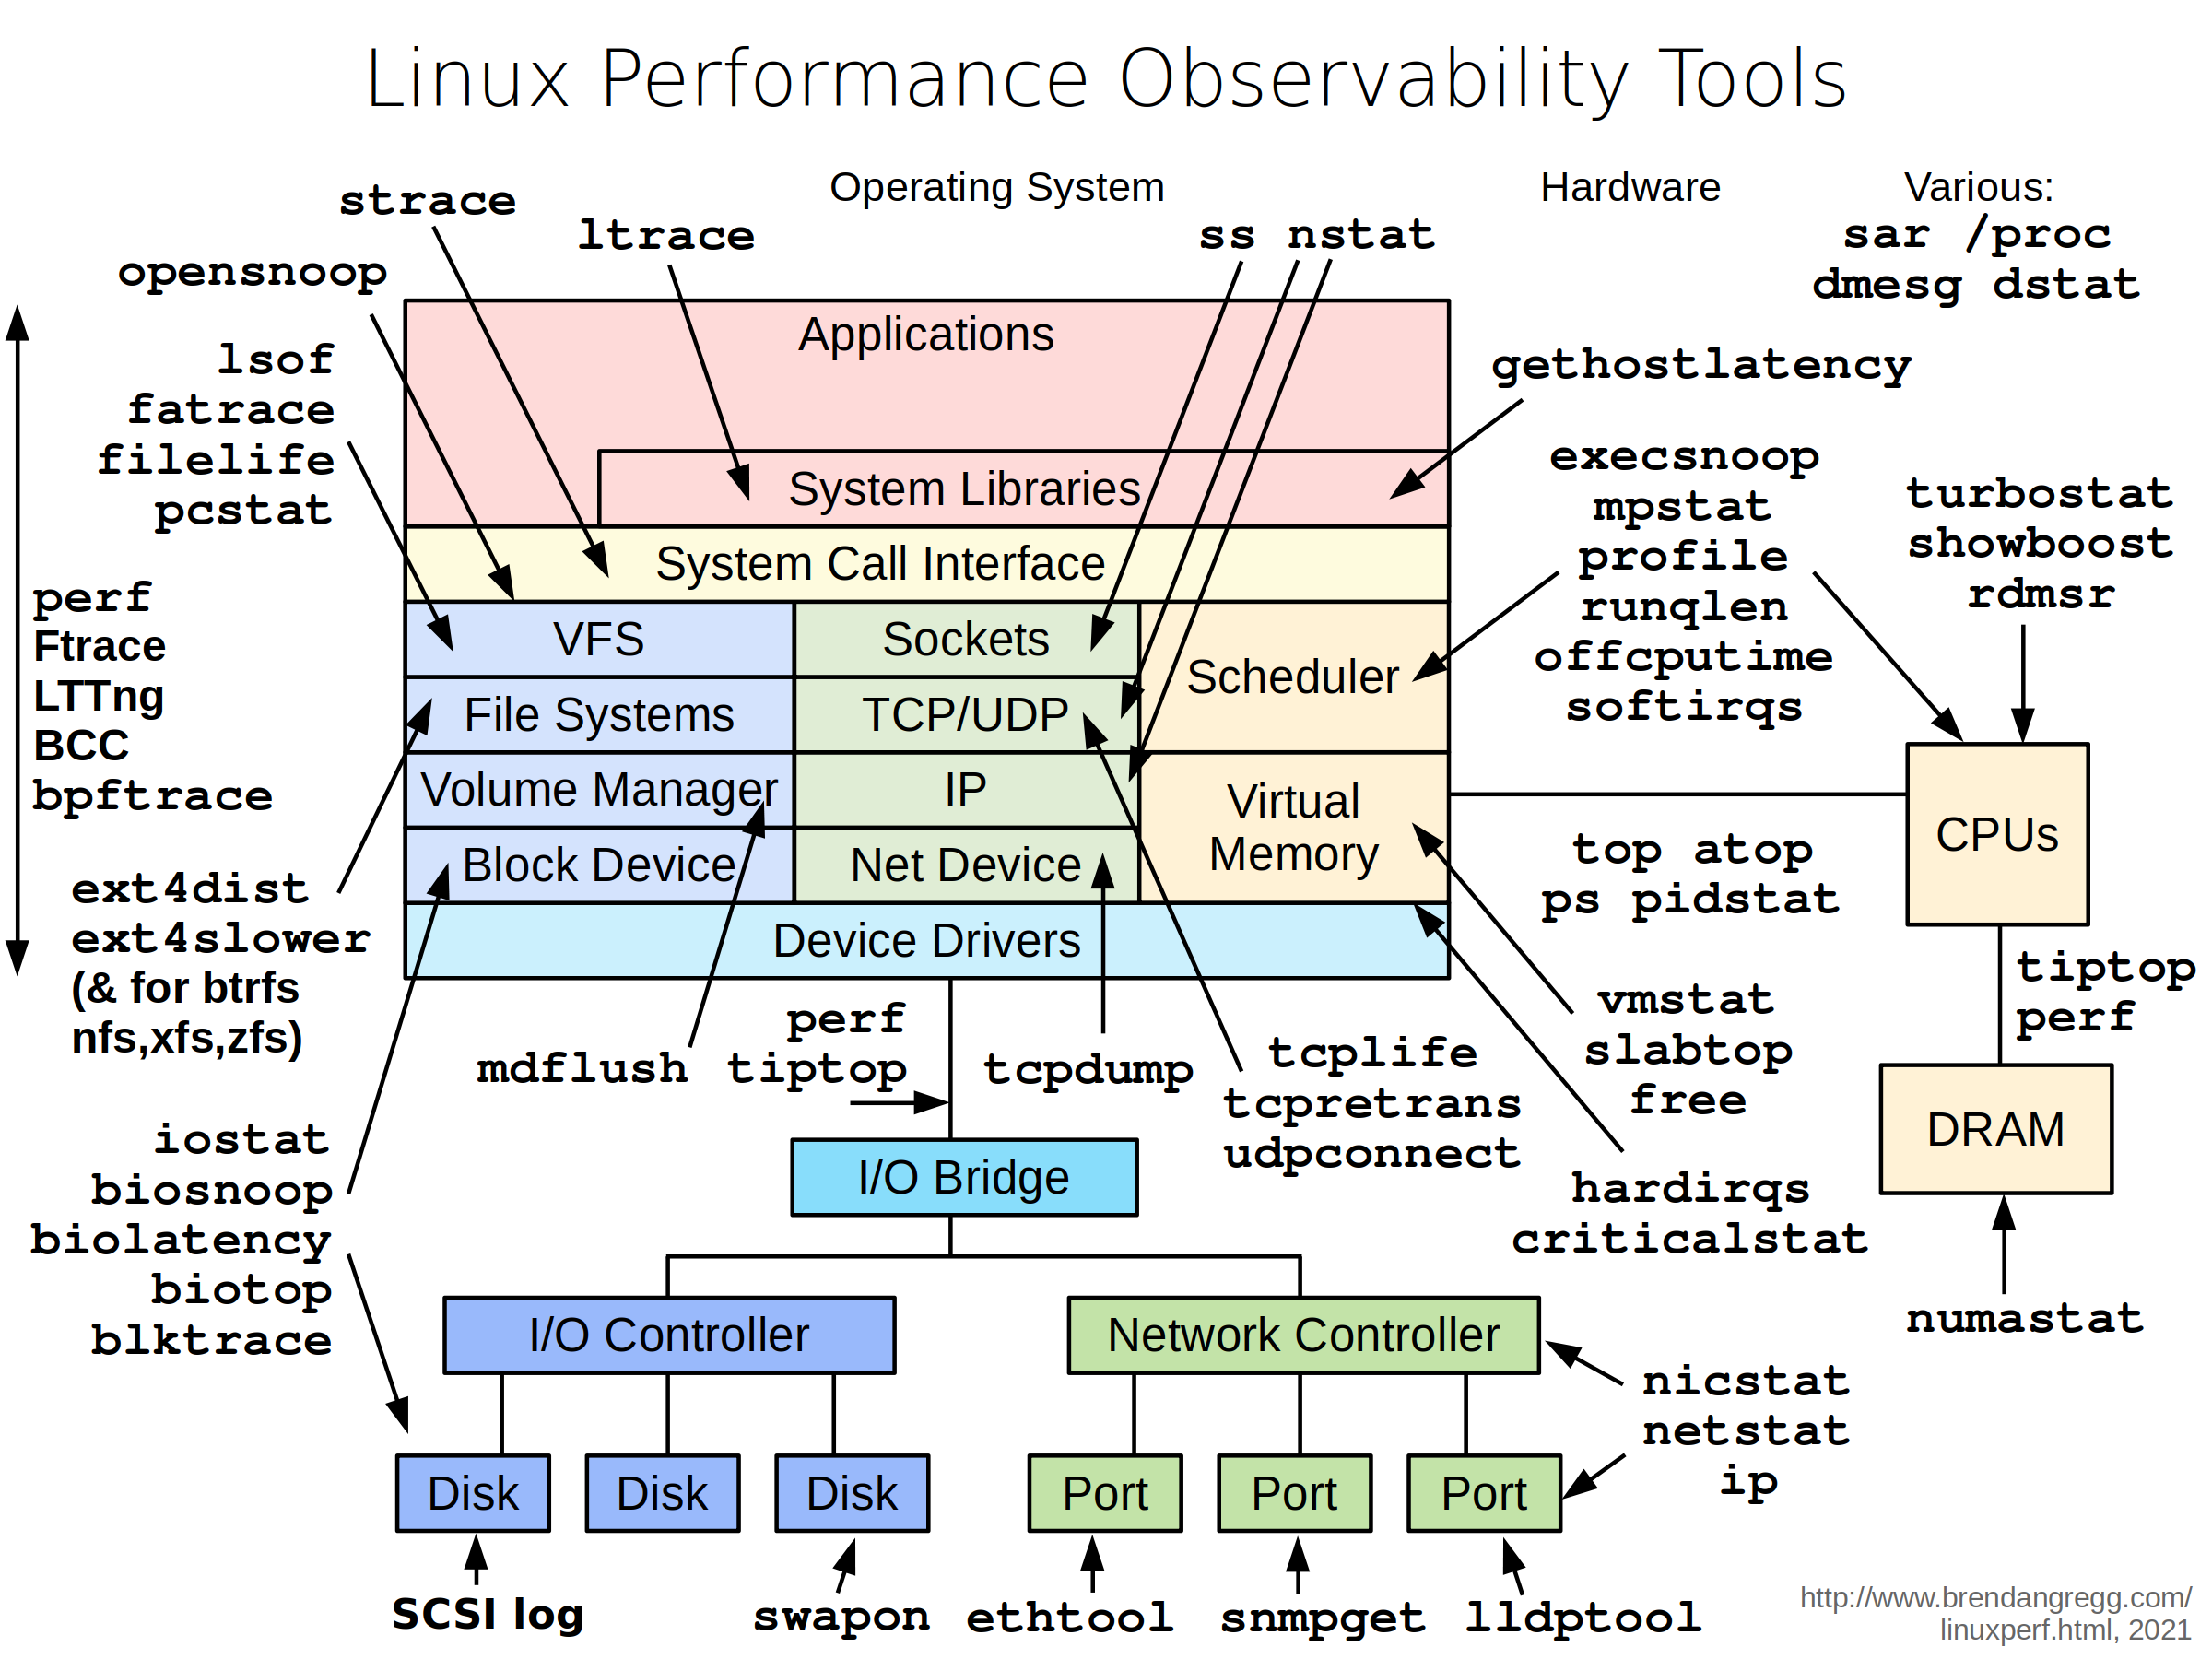
\includegraphics[width=0.6\textwidth]{img/linux_observability_tools.png}
    \end{center}
\end{frame}

\begin{frame}{Profiling Categories}
      \begin{itemize}
          \item \textbf{System}: Overall system performance, focus on memory bandwidth, peak float performance, etc.
          \item \textbf{Program}: Focus on specific program behavior, e.g., memory access patterns, branch prediction, etc.
      \end{itemize}
   
\end{frame}

\begin{frame}{Profiling Categories}
    \textbf{Why do we need both?}
    \begin{itemize}
        \item System profiling gives us details about the hardware and the optimization upper bound(or how to build a more powerful system)
        \item Program profiling makes us able to touch the machine's limits
    \end{itemize}
\end{frame}

\begin{frame}{System Profiler Recommandation}
    \begin{columns}
        \begin{column}{0.5\textwidth}
            \begin{itemize}
                \item \textbf{CPUFP}: A tool for measuring the peak performance of kinds of SIMD instructions
                \item \footnotesize{\url{https://github.com/pigirons/cpufp}}
            \end{itemize}
        \end{column}
        \begin{column}{0.5\textwidth}
            \centering
            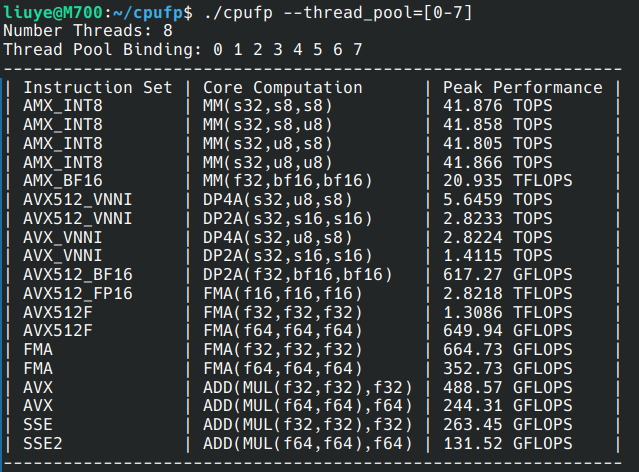
\includegraphics[width=\textwidth]{img/cpufp.png}
        \end{column}
    \end{columns}
\end{frame}

\begin{frame}{System Profiler Recommandation}
    \begin{columns}
        \begin{column}{0.5\textwidth}
            \begin{itemize}
                \item \textbf{core-to-core-latency}: A tool for measuring the latency of core communication
                \item \footnotesize{\url{https://github.com/nviennot/core-to-core-latency}}
            \end{itemize}
        \end{column}
        \begin{column}{0.5\textwidth}
            \centering
            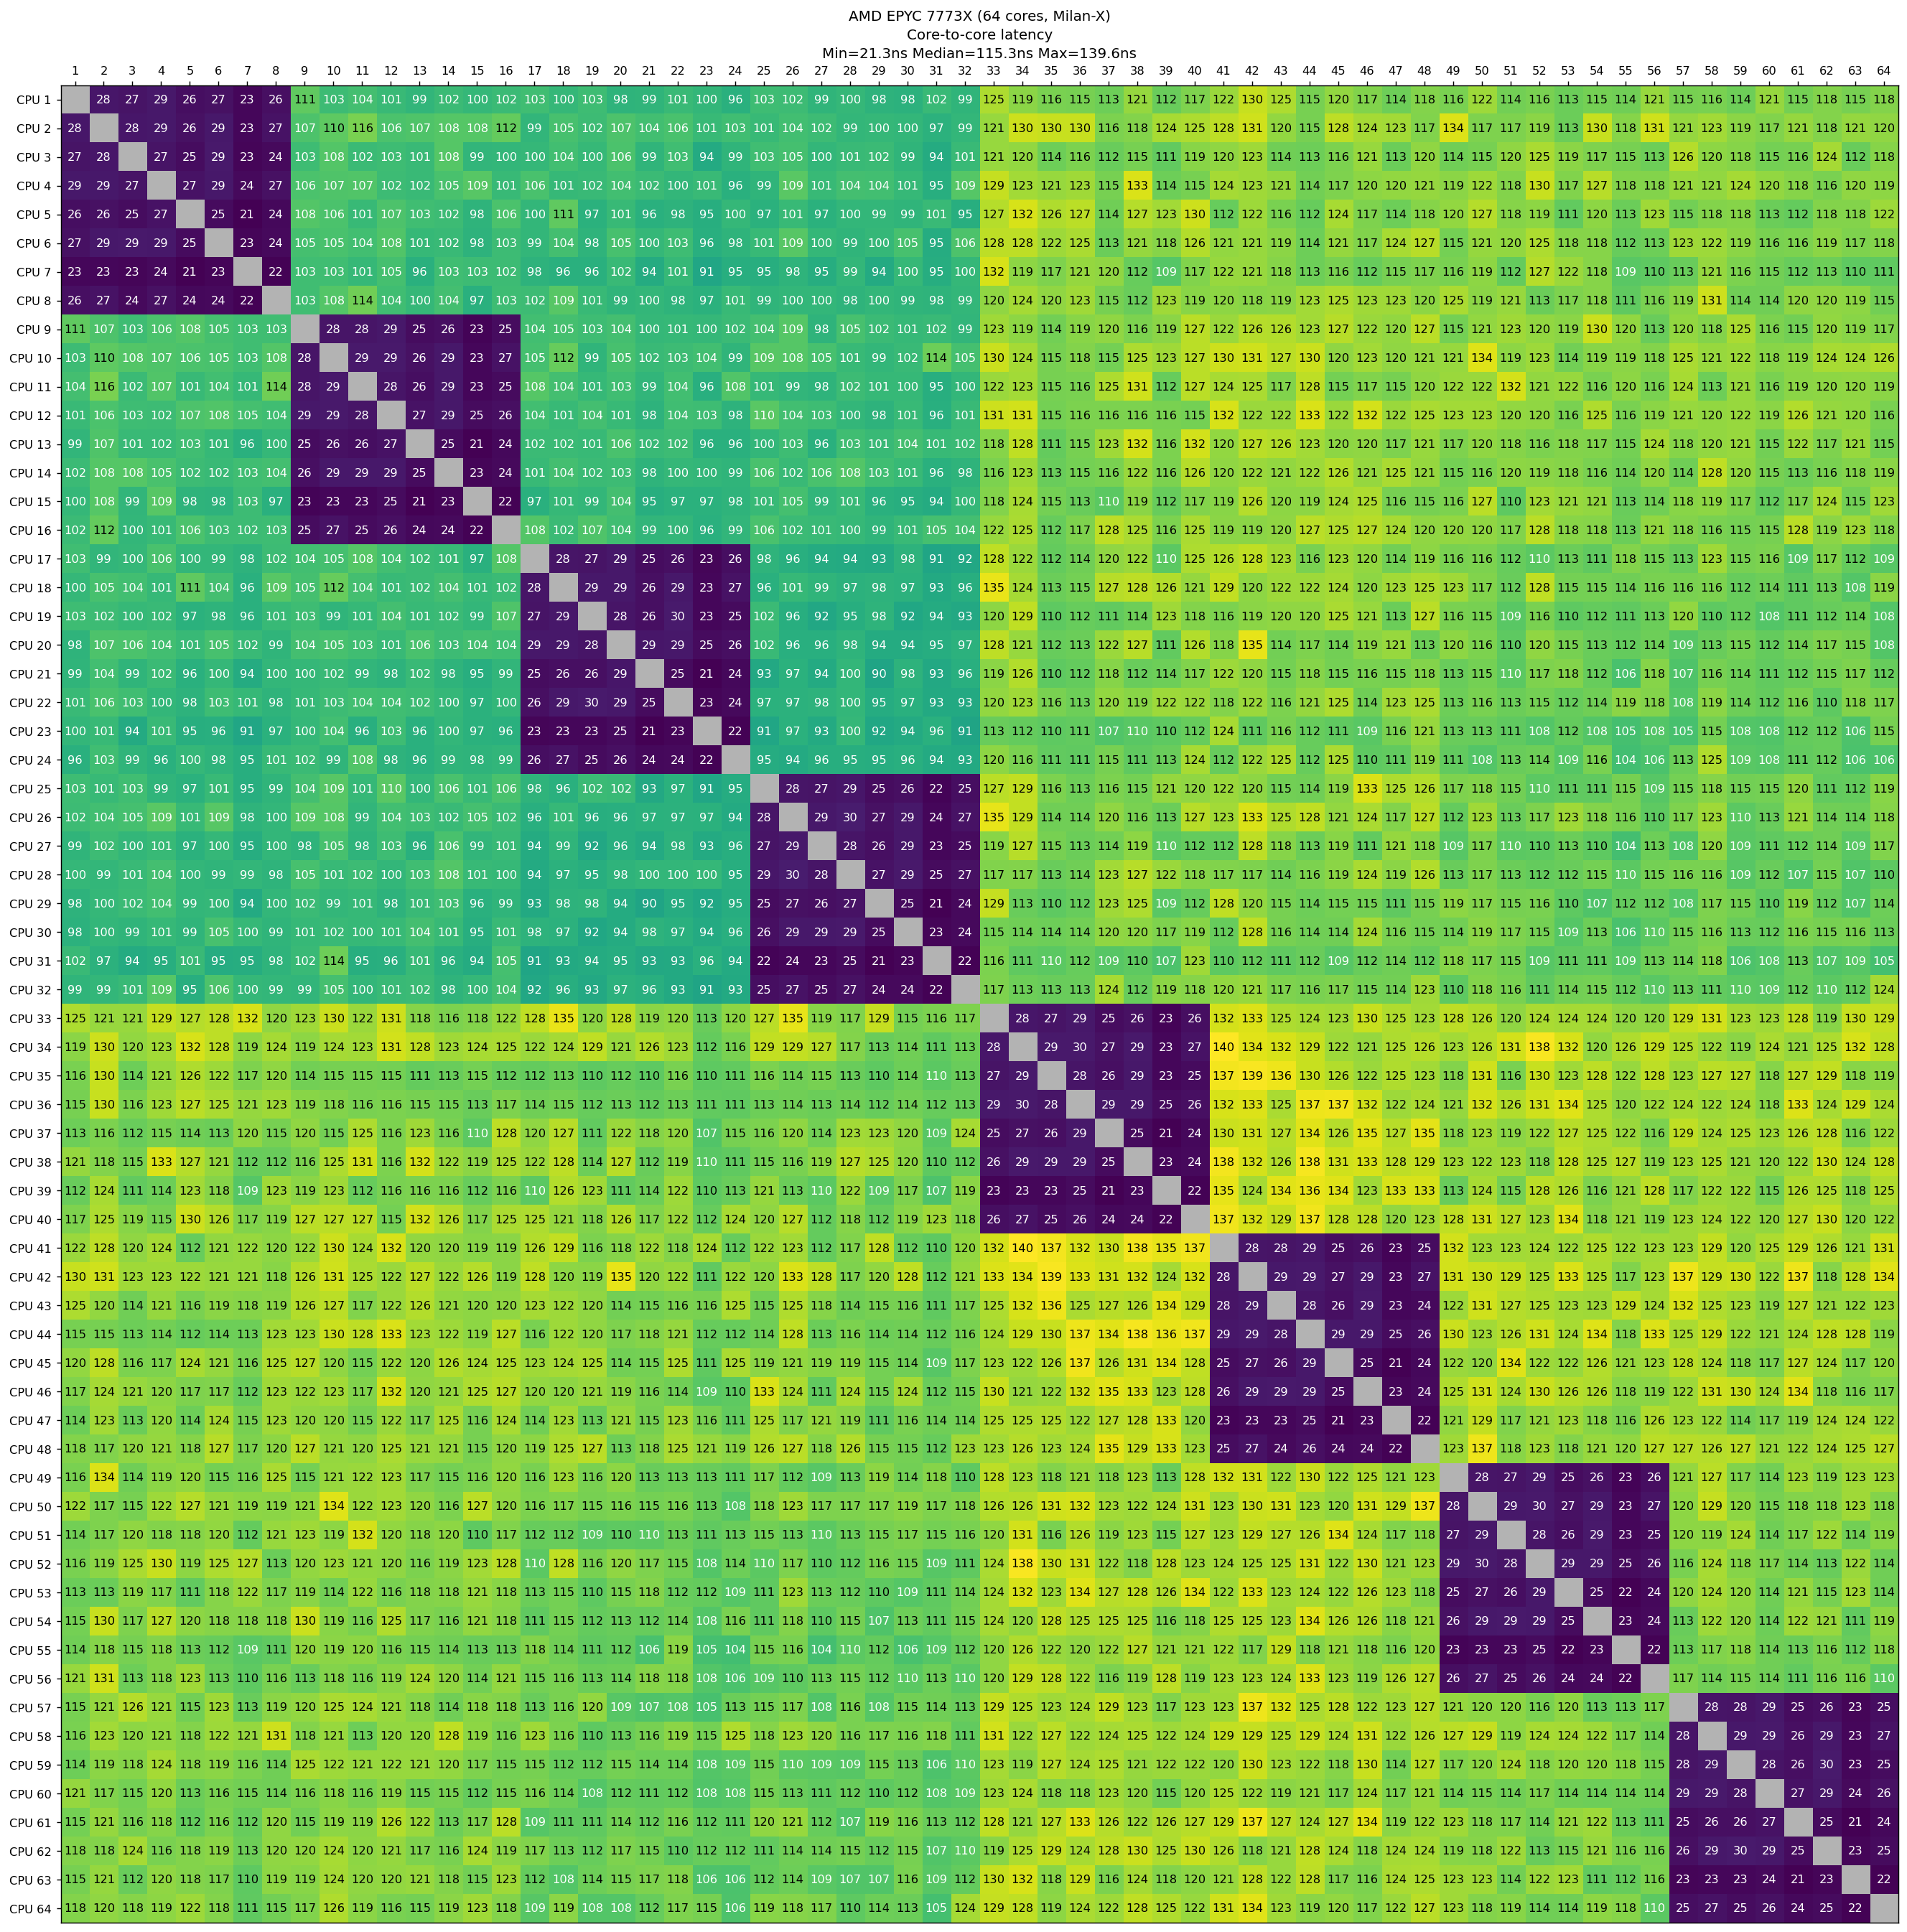
\includegraphics[width=\textwidth]{img/core2core.png}
        \end{column}
    \end{columns}
\end{frame}

\begin{frame}{System Profiler Recommandation}
    \begin{columns}
        \begin{column}{0.5\textwidth}
            \begin{itemize}
                \item \textbf{STREAM}: A tool for measuring the memory bandwidth
                \item \footnotesize{\url{https://github.com/jeffhammond/STREAM}}
            \end{itemize}
        \end{column}
        \begin{column}{0.5\textwidth}
            \centering
            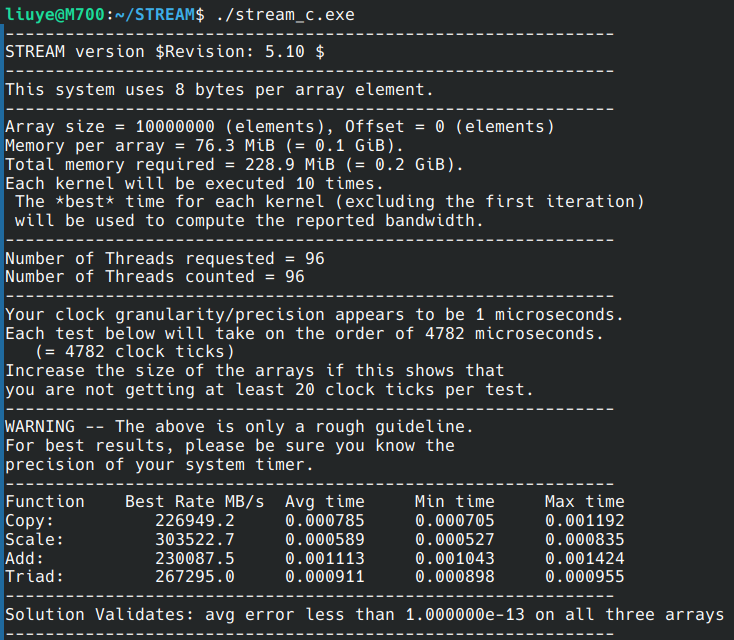
\includegraphics[width=\textwidth]{img/stream.png}
        \end{column}
    \end{columns}
\end{frame}

\begin{frame}{System Profiler Recommandation}
    \begin{columns}
        \begin{column}{0.5\textwidth}
            \begin{itemize}
                \item \textbf{cpu-micro-benchmark}: A tool for reverse engineering CPU microarchitecture
                \item \footnotesize{\url{https://github.com/jiegec/cpu-micro-benchmarks}}
                \item \footnotesize{\url{https://jia.je/hardware/2024/12/27/cpu-uarch-reverse-engineering-methodology}}
            \end{itemize}
        \end{column}
        \begin{column}{0.5\textwidth}
            \centering
            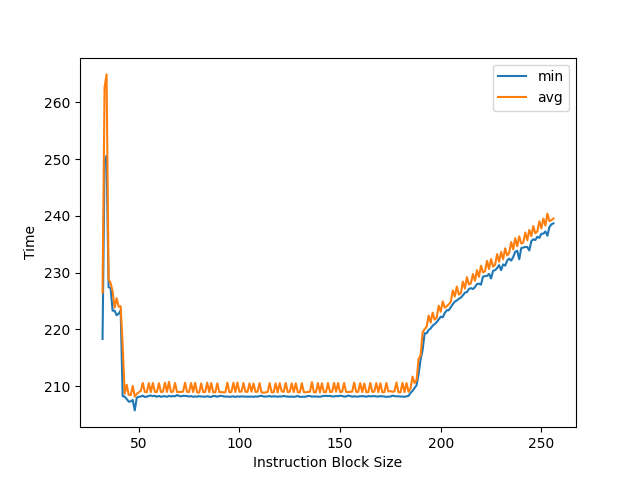
\includegraphics[width=\textwidth]{img/intel_broadwell.png}
        \end{column}
    \end{columns}
\end{frame}